\documentclass{article}
\usepackage{nips10submit_e,times}

\title{Online variational inference for state-space models with point process observations}

	
\usepackage[dvips]{epsfig}
\usepackage{url}
\usepackage{amsmath}
\usepackage{amsfonts}
\usepackage{amssymb}
%\usepackage{graphicx}
\usepackage{bm}
\usepackage{array}
\usepackage{subfigure}
\usepackage{float}
\floatstyle{ruled}
\newfloat{algorithm}{htbp}{loa}[section]
\floatname{algorithm}{Algorithm}

\newcolumntype{x}[1]{%
>{\centering\hspace{0pt}}p{#1}}%

\newcounter{remarkcounter}
%\addtocounter{remarkcounter}{1}

\newtheorem{theorem}{Theorem}
\newtheorem{lemma}[theorem]{Lemma}
\newtheorem{proposition}[theorem]{Proposition}
\newtheorem{corollary}[theorem]{Corollary}
\newtheorem{remark}[remarkcounter]{Remark}


\newenvironment{proof}[1][Proof]{\textbf{#1.} }{\ \rule{0.5em}{0.5em}}
\newenvironment{definition}[1][Definition]{\begin{trivlist}
\item[\hskip \labelsep {\bfseries #1}]}{\end{trivlist}}
\newenvironment{example}[1][Example]{\begin{trivlist}
\item[\hskip \labelsep {\bfseries #1}]}{\end{trivlist}}
%\newenvironment{remark}[1][Remark]{\begin{trivlist}
%\item[\hskip \labelsep {\bfseries #1}]}{\end{trivlist}}

\newcommand{\Azero} {\textsl{} A}
\newcommand{\Bzero} {\textsl{} B_0}
\newcommand{\Tkk} {{\bf T}_{k-1}}
\newcommand{\Jk} {{\bf J}_{k}}
\newcommand{\Ak} {{\bf A}_k}
\newcommand{\Akplusone} {{\bf A}_{k+1}}
\newcommand{\Akk} {{\bf A}_{k-1}}
\newcommand{\Amat} {{\bf A}}
\newcommand{\Cmat} {{\bf C}}
\newcommand{\thetab} {{\bm \theta}}
\newcommand{\chib} {{\bm \chi}}
\newcommand{\rhob} {{\bm \rho}}
\newcommand{\thetabj} {{\bm \theta}_j}
\newcommand{\thetabjj} {{\bm \theta}_{j-1}}
\newcommand{\thetabk} {{\bm \theta}_k}
\newcommand{\thetabkk} {{\bm \theta}_{k-1}}
\newcommand{\thetabkkk} {{\bm \theta}_{k-2}}
\newcommand{\thetabkkkk} {{\bm \theta}_{k-3}}
\newcommand{\thetabkkhat} {{\hat{\bm \theta}}_{k-1}}
\newcommand{\thetabkkkhat} {{\hat{\bm \theta}}_{k-2}}
\newcommand{\thetabkkkkhat} {{\hat{\bm \theta}}_{k-3}}
\newcommand{\Thetak} {\Theta_{k}}
\newcommand{\Thetakk} {\Theta_{k-1}}
\newcommand{\Thetakkk} {\Theta_{k-2}}
\newcommand{\phib} {{\bm \phi}}
\newcommand{\psib} {{\bm \psi}}
\newcommand{\zetab} {{\bm \zeta}}
\newcommand{\zetabk} {{\bm \zeta}_k}
\newcommand{\Phib} {{\bm \Phi}}
\newcommand{\z} {{\bf z}}
\newcommand{\un} {{\bf u_n}}
\newcommand{\s} {{\bf s}}
\newcommand{\rr} {{\bf r}}
\newcommand{\ab} {{\bf a}}
\newcommand{\aj} {{\bf a}_j}
\newcommand{\ai} {{\bf a}_i}
\newcommand{\aik} {{\bf a}_{i,k}}
\newcommand{\ajk} {{\bf a}_{j,k}}
\newcommand{\ajzero} {{\bf a}_{j,0}}
\newcommand{\aikk} {{\bf a}_{i,{k-1}}}
\newcommand{\ajkk} {{\bf a}_{j,{k-1}}}
\newcommand{\ajkkk} {{\bf a}_{j,{k-2}}}
\newcommand{\ajkplusone} {{\bf a}_{j,k+1}}
\newcommand{\ajkgivenk} {{\bf a}_{j,k|k}}
\newcommand{\ajkkgivenkk} {{\bf a}_{j,k-1|k-1}}
\newcommand{\sjk} {{\bf s}_{j,k}}
\newcommand{\x} {{\bf x}}
\newcommand{\e} {{\bf e}}
\newcommand{\w} {{\bf w}}
\newcommand{\W} {{\bf W}}
\newcommand{\y} {{\bf y}}
\newcommand{\q} {{\bf q}}
\newcommand{\Ik} {{\bf I}_k}
\newcommand{\ub} {{\bf u}}
\newcommand{\Qm} {{\mathcal{Q}}}
\newcommand{\mub} {{\bm \mu}}
\newcommand{\mubk} {{\bm \mu_k}}
\newcommand{\mubkk} {{\bm \mu_{k-1}}}	
\newcommand{\mubkoff} {{\bm \mu_k'}}
\newcommand{\mubkkoff} {{\bm \mu_{k-1}'}}
\newcommand{\mubAkk} {{\bm \mu^A_{k-1}}}
\newcommand{\mubAkkk} {{\bm \mu^A_{k-2}}}
\newcommand{\mubAjk} {{\bm \mu^A_{j,k}}}
\newcommand{\mubAjkk} {{\bm \mu^A_{j,k-1}}}
\newcommand{\mubAjkkk} {{\bm \mu^A_{j,k-2}}}
\newcommand{\mubktilde} {\widetilde{\bm \mu_k}}
\newcommand{\mubthetakk} {{\bm \mu^{\thetab}_{k-1}}}
\newcommand{\mubthetakkk} {{\bm \mu^{\thetab}_{k-2}}}
\newcommand{\vv} {{\bm \nu}}
\newcommand{\vvm} {{\mathcal {\bm \upsilon}}}
\newcommand{\kappab} {{\mathcal {\bm \kappa}}}
\newcommand{\alphainv} {\alpha^{-1}}
\newcommand{\Jcost} {{\mathcal J}}
\newcommand{\xdot} {{\bf \dot{x}}}
\newcommand{\Vm} {{\bf \mathcal{V}}}
\newcommand{\expect} {\mathbb{E}}
\renewcommand{\Re} {\mathbb{R}}
\newcommand{\Var} {\mathrm{Var}}
\newcommand{\N} {\mathcal{N}}
\newcommand{\Zplus} {\mathbb{Z}^+}
\newcommand{\ltheta} {{l_\thetab}}
%\renewcommand{\int} {\int}

\newcommand{\Psixinv} {{\bf \Psi_x^{-1}}}
\newcommand{\Psix} {{\bf \Psi_x}}
\newcommand{\Psie} {{\bf \Psi_e}}
\newcommand{\Psitheta} {{\bf \Psi_\theta}}
\newcommand{\Sigmawinv} {{\bf \Sigma_w^{-1}}}
\newcommand{\Sigmaw} {{\bf \Sigma_w}}
\newcommand{\SigmaA} {{\bf \Sigma_A}}
\newcommand{\Sigmamu} {{\bf \Sigma_{\mu}}}
\newcommand{\Sigmarho} {{\bf \Sigma_{\rho}}}
\newcommand{\Sigmaalpha} {{\bf \Sigma_{\alpha}}}
\newcommand{\Sigmarhohat} {{\bf \hat{\Sigma_{\rho}}}}
\newcommand{\Sigmab} {{\bf \Sigma}}
\newcommand{\Sigmabk} {{\bf \Sigma_k}}
\newcommand{\Sigmabktilde} {\widetilde{\bf \Sigma_k}}
\newcommand{\Sigmakk} { \Sigma_{k-1}}
\newcommand{\Sigmakkinv} { \Sigma_{k-1}^{-1}}
\newcommand{\Sigmabkk} {{\bf \Sigma_{k-1}}}
\newcommand{\Sigmabkkstar} {{\bf \Sigma_{k-1}^*}}
\newcommand{\Sigmabkinv} {{\bf \Sigma_k^{-1}}}
\newcommand{\Sigmabkkinv} {{\bf \Sigma_{k-1}^{-1}}}
\newcommand{\Sigmabkoff} {{\bf \Sigma_k'}}
\newcommand{\Sigmabkoffinv} {{\bf \Sigma_{k}'^{-1}}}
\newcommand{\Sigmabkkoff} {{\bf \Sigma_{k-1}'}}
\newcommand{\Sigmabkkoffinv} {{\bf \Sigma_{k-1}'^{-1}}}
\newcommand{\Sigmabthetakk} {{\bf \Sigma^{\thetab}_{k-1}}}
\newcommand{\Sigmabek} {{\bf \Sigma^{e}_{k}}}
\newcommand{\Sigmabekk} {{\bf \Sigma^{e}_{k-1}}}
\newcommand{\Sigmabekkk} {{\bf \Sigma^{e}_{k-2}}}
\newcommand{\Sigmabthetakkinv} {{\bf \Sigma^{\thetab^{-1}}_{k-1}}}
\newcommand{\Sigmabthetakkkinv} {{\bf \Sigma^{\thetab^{-1}}_{k-2}}}
\newcommand{\Sigmabthetakkk} {{\bf \Sigma^{\thetab}_{k-2}}}
\newcommand{\Sigmav} {{\bf \Sigma_v}}
\newcommand{\betab} {{\bm \beta}}
\newcommand{\gammab} {{\bm \gamma}}

\newcommand{\A}{{\bf A}}
\newcommand{\Astar}{{\bf A^*}}
\newcommand{\Atilde}{{\bf \tilde{A}}}
\newcommand{\Ahat}{{\bf \hat{A}}}
\newcommand{\ba}{{\bf a}}
\newcommand{\B}{{\bf B}}
\newcommand{\E}{{\bf E}}
\newcommand{\D}{{\bf D}}
\newcommand{\F}{{\bf F}}
\newcommand{\FF}{{\mathcal F}}
\newcommand{\OO}{{\mathcal O}}

\newcommand{\bb}{{\bf b}}
\newcommand{\f}{{\bf f}}
\newcommand{\ft}{\tilde{f}}
\newcommand{\pt}{\tilde{p}}
\newcommand{\phat}{\hat{p}}
\newcommand{\h}{{\bf h}}
\newcommand{\bu}{{\bf u}}
\newcommand{\ud}{{\bf u_d}}
\newcommand{\bv}{{\bf v}}
\newcommand{\zk}{{\bf z_k}}
\newcommand{\zkk}{{\bf z_{k-1}}}
\newcommand{\C}{{\bf C}}
\newcommand{\CA}{{\bf C^A}}
\newcommand{\Ck}{{\bf C}_k}
\newcommand{\Ckk}{{\bf C}_{k+1}}
\newcommand{\I}{{\bf I}}
\newcommand{\G}{{\bf G}}
\newcommand{\Sk}{{\bf S}_k}
\newcommand{\Wk}{{\bf W}_k}
\newcommand{\Wkk}{{\bf W}_{k-1}}
\newcommand{\Z}{{\bf Z}}
\newcommand{\Hk}{{\bf H_k}}
\newcommand{\Q}{{\bf Q}}
\newcommand{\Qinv}{{\bf Q}^{-1}}
\newcommand{\Qdinv}{{\bf Q}^{-2}}
\newcommand{\R}{{\bf R}}
\newcommand{\Rinv}{{\bf R}^{-1}}
\newcommand{\Kk}{{\bf K_k}}
\newcommand{\Kkplusone}{{\bf K_{k+1}}}
\newcommand{\Y}{\mathcal{Y}}
\newcommand{\Yj}{\mathcal{Y}_j}
\newcommand{\Yk}{\mathcal{Y}_k}
\newcommand{\Ykk}{\mathcal{Y}_{k-1}}
\newcommand{\Ykkk}{\mathcal{Y}_{k-2}}
\newcommand{\X}{\mathcal{X}}
\newcommand{\Xk}{\mathcal{X}_k}
\newcommand{\Xkk}{\mathcal{X}_{k-1}}
\newcommand{\Xkkk}{\mathcal{X}_{k-2}}
\newcommand{\Xkkkk}{\mathcal{X}_{k-3}}
\newcommand{\Asetk}{\mathcal{A}_k}
\newcommand{\Asetkk}{\mathcal{A}_{k-1}}
\newcommand{\zero}{{\bf 0}}
\newcommand{\Thetahatkk}{{\hat{\Theta}_{k-1}}}
\newcommand{\Thetahatkkk}{{\hat{\Theta}_{k-2}}}
\newcommand{\Thetahatkkkk}{{\hat{\Theta}_{k-3}}}


\newcommand{\xstar}{{\bf x^*}}
\newcommand{\Dx}{{\bf \Delta x}}
\newcommand{\Dxdot}{{\bf \Delta \dot{x}}}
\newcommand{\xj}{{\bf x}_j}
\newcommand{\xjj}{{\bf x}_{j-1}}
\newcommand{\xk}{{\bf x}_k}
\newcommand{\xkk}{{\bf x}_{k-1}}
\newcommand{\xkkk}{{\bf x}_{k-2}}
\newcommand{\xkkkk}{{\bf x}_{k-3}}
\newcommand{\ek}{{\bf e}_k}
\newcommand{\ekk}{{\bf e}_{k-1}}
\newcommand{\yk}{{\bf y}_k}
\newcommand{\ykk}{{\bf y}_{k-1}}
\newcommand{\uk}{{\bf u}_k}
\newcommand{\wk}{{\bf w}_k}
\newcommand{\vk}{{\bf v}_k}
\newcommand{\Pk}{{\bf P}_k}
\newcommand{\Pkplusone}{{\bf P}_{k+1}}
\newcommand{\xkplusone}{{\bf x}_{k+1}}
\newcommand{\xkprev}{{\bf x}_{k-1}}

\newcommand{\wkprev}{{\bf w}_{k-1}}
\newcommand{\vkprev}{{\bf v}_{k-1}}
\newcommand{\xhat}{{\bf \hat{x}}}
\newcommand{\xkhat}{{\bf \hat{x}}_k}
\newcommand{\xkhatprev}{{\bf \hat{x}}_{k-1}}
\newcommand{\xktilde}{{\bf \widetilde{x}}_k}
\newcommand{\ekprior}{{\bf e_{k}^-}}
\newcommand{\ekpriorplusone}{{\bf e}_{k+1}^{-}}
\newcommand{\Pkprior}{{\bf P_{k}^-}}
\newcommand{\Pkpriorplusone}{{\bf P}_{k+1}^-}
\newcommand{\xkhatprior}{{\bf \hat{x}}_k^-}
\newcommand{\xkhatpriorplusone}{{\bf \hat{x}}_{k+1}^-}
\newcommand{\xzerohatprior}{{\bf \hat{x}}_0^-}
\newcommand{\Pzeroprior}{{\bf P}_{0}^-}

\newcommand{\xhatatkgivenk}{{\bf \hat{x}}_{k \mid k}}
\newcommand{\xhatatkkgivenk}{{\bf \hat{x}}_{k-1 \mid k}}
\newcommand{\xhatatkkgivenkk}{{\bf \hat{x}}_{k-1 \mid k-1}}
\newcommand{\xhatatkgivenN}{{\bf \hat{x}}_{k \mid N}}
\newcommand{\xhatatNgivenN}{{\bf \hat{x}}_{N \mid N}}
\newcommand{\xhatatkplusNgivenk}{{\bf \hat{x}}_{k + N \mid k}}
\newcommand{\xhatatkplusonegivenN}{{\bf \hat{x}}_{k + 1 \mid N}}
\newcommand{\xhatatkplusonegivenk}{{\bf \hat{x}}_{k + 1 \mid k}}
\newcommand{\Patkgivenk}{{\bf {P}}_{k \mid k}}
\newcommand{\PatkgivenN}{{\bf {P}}_{k \mid N}}
\newcommand{\PatNgivenN}{{\bf {P}}_{N \mid N}}
\newcommand{\PatkplusNgivenk}{{\bf {P}}_{k + N \mid k}}
\newcommand{\Patkplusonegivenk}{{\bf {P}}_{k + 1 \mid k}}
\newcommand{\PatkplusonegivenN}{{\bf {P}}_{k + 1 \mid N}}

\newcommand{\ent}{\mathcal{H}}
\newcommand{\info}{\mathcal{I}}

\newcommand{\obsmodel}{f(\yk | \thetabk,\Ykk)}
\newcommand{\evolmodel}{f(\thetabk | \thetabkk)}
\newcommand{\filterdist}{f(\thetabk | \Yk)}
\newcommand{\predictdist}{f(\thetabk | \Ykk)}
\newcommand{\smoothdist}{f(\thetabkk | \Yk)}


\usepackage{color}
\newcommand{\red}{\textcolor{red}}
\newcommand{\blue}{\textcolor{blue}}
\newcommand{\green}{\textcolor{green}}
\bibliographystyle{IEEEtran}	



\newcommand{\fix}{\marginpar{FIX}}
\newcommand{\new}{\marginpar{NEW}}


\begin{document}

\author{
Andrew Zammit Mangion \\
Department of Automatic Control and Systems Engineering\\
University of Sheffield\\
Sheffield, U.K. \\
\texttt{A.Zammit@sheffield.ac.uk} \\
\And
Ke Yuan\\
School of Electronics and Computer Science\\
University of Southampton\\
Southampton, U.K.\\
\texttt{ky08r@ecs.soton.ac.uk} \\
\AND
Visakan Kadirkamanathan\\
Department of Automatic Control and Systems Engineering\\
University of Sheffield\\
Sheffield, U.K. \\
\texttt{visakan@sheffield.ac.uk} \\
\And
Mahesan Niranjan\\
School of Electronics and Computer Science\\
University of Southampton\\
Southampton, U.K.\\
\texttt{mn@ecs.soton.ac.uk} \\
\And
Guido Sanguinetti\\
School of Informatics\\
University of Edinburgh\\
\texttt{G.Sanguinetti@ed.ac.uk}
}

\maketitle
%\maketitle
\begin{abstract} We present a variational Bayesian approach to state and parameter inference in
	state-space models with point-process observations, a physiologically plausible model for
	signal processing of spike data. We give a derivation of the variational smoother, as well
	as an efficient online filtering algorithm which can also be used to track the change in
	physiological parameters after the application of external stimuli. We assess the model on
	simulated data, comparing the results with EM as well as Monte Carlo estimation to evaluate
	the accuracy of the proposed approach. We then show an application of the online filtering
	algorithm to a real data set of taste-response neural cells, showing that the approach can
	effectively capture dynamical changes in neural responses.  \end{abstract}
	\section{Introduction}

Many biomedical signal processing problems, such as neural spikes and  heart beats, are concerned
with discrete events in time, separated by seemingly random intervals.  They are often driven by
continuous processes relating to the organ's physiology, whose charge-and-fire  type behaviour
results in observed discrete  events. Conventional approaches to  modelling such signals are largely
based on modelling the time intervals between these discrete events, which, as continuous variables,
are amenable to standard signal processing and system identification
approaches~\cite{Ivanov_1996,Jolivet_2008}.

An alternative approach is the state space model with point process observations (SSPP) recently
proposed by Smith and Brown \cite{Smith_2003}, which avoids the somewhat artificial change to
inter-spike times and handles directly the discrete events. This model assumes a first order
autoregressive process driven by an exogeneous stimulus as state dynamics and a parameterized
intensity function of a Poisson process as its observation model. For simultaneous estimation of
state and parameters of such a model, Smith and Brown derived an Expectation-Maximization (EM)
algorithm, along the lines of similar formulations \cite{Roweis_1999}.  In a recent study
\cite{Yuan_2010}, it was shown that the expectation of the log complete data likelihood
($Q$-function) of the SSPP model is unimodal and highly non-Gaussian with respect to each of its
parameters. The high skewness is indicative of parameter posteriors where simple maximum likelihood
estimates of the parameters may be quite far from the actual posterior means, motivating a Bayesian
treatment of the SSPP model. In this paper, we propose a variational Bayesian approach to solve this
problem, extending results of \cite{Beal_2003b} to the SSPP case to obtain a variational smoother
which offers a good compromise between distributional accuracy and computational efficiency. We
demonstrate our approach on a synthetic data set, showing good performance when compared to EM and
fully Bayesian approaches based on Gibbs sampling. We also provide an on-line filter using ideas
taken from dual filtering \cite{Haykin_2001}, whereby parameters are allowed to evolve to track
changes in the system's mode of operation. We present a case study based on real data of neural
responses to different taste stimuli \cite{Lorenzo_2003}, showing that the online filter correctly
predicts a change in the input gain or the background firing rate parameters when the input stimulus
is changed.  \section{Model and Inference}

We are concerned with event-based models where  we record $0 < u_1^c < u_2^c <, \dots  \le T, c = 1
\dots C$ successive events from $C$ separate output channels in an observation interval (0,$T$]. The
observation length is discretised with a sampling interval $\Delta > 0$ so that these events can be
represented as a sequence of binary vectors $\yk := \y(k\Delta) \in \Re^C$ where $y^c(k\Delta) = 1$
indicates that an event has occurred at the $c^{th}$ output channel at time $k\Delta$ and is zero
otherwise. The sampling interval $\Delta$ is chosen small enough so that at most one event per
output channel per sample is present.  The event probability in the $k$-th time interval in the
$c$-th channel conditioned on the latent state $x_k$ (observation model or likelihood) is given by
\begin{equation} p(y^c_k \mid x_k) = [\Delta \lambda^c_k]^{y^c_k}\exp(-\Delta
	\lambda^c_k)\label{spikeLike} \end{equation} where $\lambda^c_k = \exp(\mu + \beta^c x_k)$,
	which can be recognised as a discrete time approximation to an inhomogeneous Poisson point
	process (see {\em e.g.}~\cite{Daley_2003}). The parameter $\mu$ represents a background
	firing rate, which for simplicity we assume to be the same for all channels. We assume that
	the underlying state $x_k$ follows the standard linear evolution equation

\begin{equation} x_k = \rho x_{k-1} + \alpha I_k + \epsilon_k \end{equation}

\noindent where $I_k$ is 1 if an input is present at $k\Delta$ and zero otherwise. $\epsilon_k \in
\Re$ is additive white Gaussian noise with mean 0 and variance $\sigma^2_\epsilon \in \Re$. The
parameters $\rho \in \Re$ and $\alpha \in \Re$ are the propagation constant and input gain
respectively.  This model was introduced in \cite{Smith_2003} as a physiologically plausible model
of induced neural spiking experiments (see {\em e.g.} \cite{Ergun_2007}).

In practice, both the parameters governing the firing rate $\mu$ and $\betab = \{\beta^c\}_{c=1}^C$,
and the governing state equation parameters $\alpha$ and $\rho$ are unknown. We are hence faced with
the problem of having to estimate a set of unknown parameters $\thetab \in \Re^d, d = c+3$ with
$\thetab = \{\alpha,\rho,\mu,\betab\}$ in addition to an underlying hidden state $x_k$.

\subsection{The variational posteriors}

The variational framework for the inference in the SSPP model is developed in a similar way to
\cite{Beal_2003b}. Let $\X_K, \Y_K$ be the set of states and observed data points up to the final
time point $K = T/\Delta$ respectively, $\X_K = \{x_i\}_{i=1}^K$ and $\Y_K = \{\y_i\}_{i=1}^K$. We
wish to find an approximation to the true posterior $p(\X_K,\thetab | \Y_K) \approx
\pt(\X_K,\thetab)$ which maximises the variational free energy~\cite{Attias_1999}. We assume the
approximate (joint) posterior to be a product of Gaussian distributions \begin{equation}\label{eq:
	VarApproximation} \pt(\X_K,\thetab)=
	\pt(\X_K)\pt(\thetab)=\pt(\X_K)\pt(\rho|\alpha)\pt(\alpha)\pt(\mu)\prod_{i=1}^C\pt(\beta^i)
\end{equation} The dependency between the $\rho$ and $\alpha$ parameters is retained since the
interaction terms between them which appear when deriving the log posterior are relatively easy to
compute.  The optimal choice for the variational posteriors $\pt(\X_K)$ and $\pt(\thetab)$  is then
given by \begin{subequations}\label{eq:VBmarginals} \begin{align} \pt(\X_K)&\propto \exp(\langle\ln
	p(\X_K,\Y_K,\thetab)\rangle_{\pt(\thetab)}) \label{eq:xkmarginal}\\[1ex]
	\pt(\theta^i)&\propto \exp(\langle\ln
	p(\X_K,\Y_K,\thetab)\rangle_{\pt(\X_K)\pt(\thetab^{/i})}) \label{eq:thetakmarginal}
\end{align} \end{subequations} \noindent where $\theta^i$ is the $i^{th}$ component in $\thetab$ and
$\thetab^{/i}$ is the set of all $\thetab$ excluding  $\theta^i$. The notation $\langle \cdot
\rangle_{p(x)}$ denotes the expectation operator taken with respect to the distribution $p(x)$.

In the standard case of linear-Gaussian dynamical systems, the variational posteriors can be
computed exactly~\cite{Beal_2003b}. For the model we consider, because of the form of the
observation model, this is not possible. As it turns out, the observation density is unimodal, and
simulation studies have shown that it can be reasonably approximated by a Gaussian distribution. We
take advantage of this property and introduce linearisations in a way similar to~\cite{Smith_2003}
to obtain analytically tractable forward and backward passes for the state VB-E step and the
subsequent parameter updates in the VB-M step. The computations are somewhat intricate so we only present the results in the following; complete derivations are given in the supplementary material.
\subsubsection{VB-E step}\label{sec:VBE}

Evaluating (\ref{eq:xkmarginal}) and linearising as in \cite{Smith_2003}, one obtains the following
equations governing the forward pass

\begin{subequations} \begin{align} x_{k|k} = \tilde{x_k} +\tilde{\sigma}^2_k \sum_{c=1}^C
	\left\{\langle\beta^c\rangle_{\pt(\beta^c)}y^c_k - \Delta \langle \exp{\mu}
	\rangle_{\pt(\mu)} \frac{d}{dx_{k}}\left.\left[\langle \exp{x_k\beta^c}
	\rangle_{\pt(\beta^c)}\right]\right|_{x_k = x_{k | k}}  \right\} \label{eq:NL1} \\
	\sigma^2_{k|k} = \left(\tilde{\sigma}^{-2}_k + \sum_{c=1}^C \left\{\Delta  \langle \exp{\mu}
	\rangle_{\pt(\mu)} \frac{d^2}{dx_k^2}\left.\left[\langle \exp{x_k\beta^c}
	\rangle_{\pt(\beta^c)}\right]\right|_{x_k = x_{k | k}}\right\}\right)^{-1} \end{align}
\end{subequations}

\noindent where


\begin{equation}\begin{split}\label{eq:tildesa} &\frac{\tilde{x_k}}{\tilde{\sigma}^2_k}=
	\bigg((\sigma^{-2}_{k-1|k-1} + \langle \rho^2 \rangle \sigma^{-2}_\epsilon )^{-1} \langle
	\rho \rangle\sigma^{-2}_\epsilon\left[x_{k-1|k-1}\sigma^{-2}_{k-1|k-1} - \langle \rho\alpha
	\rangle I_k\sigma^{-2}_\epsilon \right] + \langle \alpha \rangle I_k\sigma^{-2}_\epsilon
	\bigg)  \\ &\tilde{\sigma}^2_k = (\sigma^{-2}_\epsilon - \langle \rho \rangle^2
	(\sigma^{-2}_{k-1|k-1} + \langle \rho^2 \rangle \sigma^{-2}_\epsilon
	)^{-1}\sigma^{-4}_\epsilon  )^{-1} \end{split}\end{equation} For conciseness, in
	(\ref{eq:tildesa})  and in some of the following equations, we omit the distributions we are
	taking expectations with respect to. The normal assumption for the variational distributions
	allow analytical computation of the expectations involved in the above equations.

In a similar fashion, we compute a backward recursion on our data to obtain variational smoothed
state estimates. The resulting equations are given as \begin{equation} x_{k|K} =
	\sigma^2_{k|K}(x_{k|k}\sigma^{-2}_{k|k} + x_{k}^*\sigma^{*^{-2}}_{k}) \qquad \sigma^2_{k|K}
	= (\sigma^{-2}_{k|k} + \sigma^{*^{-2}}_{k})^{-1} \end{equation} 	\noindent where

\[ \begin{split} &\frac{x_{k}^*}{\sigma^{*^2}_{k}} = \bigg(\langle \rho \rangle
	x'_{k+1}(\sigma^{-2}_\epsilon + \sigma^{'^{-2}}_{k+1})^{-1}
	\sigma^{-2}_\epsilon\sigma'^{-2}_{k+1} + (\sigma^{-2}_\epsilon + \sigma^{'^{-2}}_{k+1})^{-1}
	\langle \rho \rangle \langle \alpha \rangle I_{k+1}\sigma^{-4}_\epsilon - \langle \rho\alpha
	\rangle I_{k+1}\sigma^{-2}_\epsilon \bigg)\\ &\sigma^{*^2}_{k} = (\langle \rho^2
	\rangle\sigma^{-2}_\epsilon - (\sigma^{-2}_\epsilon + \sigma^{'^{-2}}_{k+1})^{-1}\langle
	\rho \rangle^2\sigma^{-4}_\epsilon )^{-1} \end{split} \] \noindent and where
	\begin{subequations} \begin{equation} \begin{array}{rcl} x'_{k+1} &=& \displaystyle
		x_{k+1|k+1} + \sigma'^2_{k+1}\frac{x_{k+1}^* - x_{k+1|k+1}}{\sigma^{2^*}_{k+1}} +
		\sum_{c=1}^C \bigg\{\langle\beta^c\rangle_{\pt(\beta^c)}y^c_{k+1} - \\[2ex] &&
		~~~~\displaystyle \Delta \langle \exp{\mu} \rangle_{\pt(\mu)}
		\frac{d}{dx_{k+1}}\left.\left[\langle \exp{x_{k+1}\beta^c}
		\rangle_{\pt(\beta^c)}\right]\right|_{x_{k+1} = x_{k+1|k+1} }  \bigg\}
		\label{eq:NL2}  \\ \end{array} \end{equation} \begin{equation} \sigma'^2_{k+1} =
			\left({\sigma}^{*^{-2}}_{k+1} + \sum_{c=1}^C \left\{\Delta  \langle
			\exp{\mu} \rangle_{\pt(\mu)} \frac{d^2}{dx_{k+1}^2}\left.\left[\langle
			\exp{x_{k+1}\beta^c} \rangle_{\pt(\beta^c)}\right]\right|_{x_{k+1} =
			x_{k+1|k+1}}\right\}\right)^{-1} \label{eq:NL2b} \end{equation}
		\end{subequations}
		
		In (\ref{eq:NL2}) and (\ref{eq:NL2b}) we have linearised around
		the filtered estimate to give a closed form solution. As a consequence of this the forward and backward passes need to be carried out	sequentially. On completing the backward pass one can update the initial state estimate $x_{1|1}$ and $\sigma^2_{1|1}$ in the same manner	as~\cite{Smith_2003}.

Equation (\ref{eq:NL1}) is not available in closed form and needs to be solved by a deterministic
optimisation method. We can take advantage of the facts that the equation has a unique solution, and
that the prior $x_{k|k-1}$ can be used as a good initialisation for $x_{k|k}$, to solve the optimisation method
in an efficient manner. In practice it was found that replacing the state variable on the right hand
side by the prior (to obtain a closed form solution) gave very good results and a marked decrease in
computational requirements.

The required statistics needed for the VB-M step are $\langle x_kx_{k+1} \rangle_{\pt(\X_K)},
\langle x_k^2 \rangle_{\pt(\X_K)}$ and $\langle x_k \rangle_{\pt(\X_K)}$ for all time $k$. The only
quantity which is not readily available from the above is the first of these expectations. To obtain
this we invert the precision matrix of the pairwise marginal $p(x_k,x_{k+1}|\Y_K)$ to obtain the following expression

\begin{equation} \langle x_kx_{k+1} \rangle_{\pt(\X_K)} = \langle \rho \rangle \sigma^{-2}_\epsilon\left((\sigma^{-2}_{k|k} + \langle \rho^2 \rangle \sigma^{-2}_\epsilon)\sigma^{l^{-2}} - \langle \rho \rangle^2 \sigma_\epsilon^{-4} \right)^{-1}+ x_{k+1|K}x_{k|K}
\end{equation}
\noindent where \begin{equation} \sigma^{l^{2}} = \left(\sigma^{*^{-2}}_{k+1} +
	\sigma^{-2}_\epsilon + \sum_{c=1}^C \left\{\Delta \langle \mu \rangle \
	\frac{d^2}{dx_{k+1}^2}\left.\left[\langle \exp{x_{k+1}\beta^c}
	\rangle_{\pt(\beta^c)}\right]\right|_{x_{k+1} = x_{k+1|K}} \right\} \right)^{-1}
\end{equation} After computing the state sufficient statistics, one can update the parameter
distributions in the VB-M step described next.

\subsubsection{VB-M step}\label{sec:VBM}

Equation (\ref{eq:thetakmarginal}) gives the updates for the parameter distributions. As a direct
consequence of the underlying linear state evolution model, the optimal variational estimates for
$\alpha$ and $\rho$ become identical to those in a linear dynamical system and so we refer the reader
to \cite{Beal_2003b} for details. The estimation of $\mu$ and $\beta^c$ is somewhat more involved.
Denoting the means and variances of $\mu$ and $\beta^c$ as $\hat{\mu}, \hat{\beta^c}$ and
$\sigma^2_\mu, \sigma^2_{\beta^c}$ respectively we have that \begin{subequations} \begin{align}
	\hat{\beta^c} = \beta^c_p + \sigma^2_{\beta^c_p}\sum_{i=1}^K \left(y^c_i\langle x_i
	\rangle_{\pt(\X_K)}- \Delta\langle \exp \mu \rangle_{\pt(\mu)} \frac{d}{d\beta^c}\left.
	\left[\langle \exp{x_{i}\beta^c}\rangle_{\pt(\X_K)}\right] \right| _{\beta^c =
	\hat{\beta}^c}  \right) \\ \sigma^2_{\beta^c} = \left(1 / \sigma^2_{\beta^c_p} +
	\Delta\langle \exp \mu \rangle_{\pt(\mu)} \sum_{i=1}^K  \left[\frac{d^2}{d\beta^{c^2}} \left.
	\langle \exp{x_i\beta^c}\rangle_{\pt(\X_K)}\right| _{\beta^c =
	\hat{\beta}^c}\right]\right)^{-1} \end{align} \end{subequations} 	\noindent and
	\begin{subequations} \begin{align} \hat{\mu} = \mu_p +
		\sigma^2_{\mu_p}\sum_{i=1}^K\sum_{c=1}^C \left(y^c_i - \Delta\exp(\hat{\mu}) \langle
		\exp(\beta^cx_i)\rangle_{\pt(\X_K)\pt(\beta^c)} \right) \\
		\sigma^2_{\mu} = \left(1 / \sigma^2_{\mu_p} + \Delta\exp(\hat{\mu})\sum_{i=1}^K
		\sum_{c=1}^C \langle \exp(\beta^cx_i)\rangle_{\pt(\X_K)\pt(\beta^c)} \right)^{-1}
	\end{align} \end{subequations} 	\noindent where the subscript $p$ denotes \emph{prior}.

All expectations in the above equations are standard except for $\langle
\exp(\beta^cx_i)\rangle_{\pt(\X_K)\pt(\beta^c)}$, which can be calculated using moment generating
functions (see supplementary material).  As is standard in a mean-field type approach, updates for
specific variables depend on the expectations of the remaining variables, leading to a natural
iterative algorithm. Convergence can be easily assessed by monitoring changes in the free energy
and/ or in the statistics of the variational distributions.  \subsection{Online VB filtering for
SSPP models}\label{sec:OL}

%In this section we briefly describe a recursive inference framework which can be employed to
%estimate the states and parameters in real-time. As will be seen, this dual filter has the
%capability to track parameters and their uncertainties online.

The above offline VB algorithm can be extended for use in an online scenario with some slight
modifications. Using a standard trick in dual filtering \cite{Haykin_2001}, we introduce a time
evolution in the parameters

\begin{equation}\label{eq:thetaevolve} \thetabk = \thetabkk + \ek \end{equation}

\noindent where $\ek \in \Re^d$ is additive white Gaussian noise with covariance $\Sigmabek \in
\Re^{d\times d}$, which is also time varying (see below). Let $\Theta_k = \{\thetab_i\}_{i=2}^{k}$.
We choose the following variational posteriors

\begin{equation} \begin{array}{rcl} \pt(\Xk,\Theta_k) &\approx& \pt(\Xk) \displaystyle \prod_{j=2}^k
	\pt(\thetab_{j}) \\[1ex] &=& \pt(\Xk)\pt(\Theta_k) \\ \end{array} \end{equation}

\noindent that is, we approximate the parameters to be conditionally independent in time. To
facilitate recursion, we further restrict the variational posteriors to be the filtered
distributions. We hence re-define $\pt(\Theta_k)$ as follows

\begin{equation}\label{eq:restriction} \pt(\Theta_k) = \displaystyle \prod_{j=2}^k
	\pt(\thetab_{j}|\Y_j) \end{equation}

At each time step the distribution $\pt(\Xk)$ and $\pt(\thetab_{k})$ are variational posteriors in
the conventional sense. We refer to $\{\pt(\thetab_{j})\}_{j=2}^{k-1}$ as the \emph{restricted}
variational posteriors, as is typical in restricted variational Bayes methods~\cite{Smidl_2006b}.
With these restrictions one can obtain the following recursive updates for both the states and the
parameters

\begin{subequations}

\begin{equation} \label{eq:Convenient} \pt(x_k) \propto\displaystyle\int{ dx_{k-1}}
	\pt(x_{k-1})\exp(\langle\ln p(x_k| x_{k-1},\thetab_k)p(\yk |
	x_k,\thetab_k)\rangle_{\pt(\thetab_k)}) \end{equation}

\begin{equation} \label{eq:Convenienttheta} \begin{array}{l} \pt(\theta^i_k)\propto\exp(\langle \ln
	p(\yk|x_k,\thetab_k) p(x_k|x_{k-1},\thetab_k)\rangle_{\pt(\Xk)\pt(\thetab_k^{/i})})  \\
	[2ex] ~~~~~~~~~~~~~~~~~~~~~~~~ \times~ \exp(\langle\ln
	p(\theta^i_k|\theta^i_{k-1})\rangle_{\pt(\theta^i_{k-1})}) ~~~ i = 1 \dots d
\end{array} \end{equation}


\end{subequations}


The above does not constitute an online algorithm in the strictest sense since (\ref{eq:Convenient})
and (\ref{eq:Convenienttheta}) are evidently coupled, and, as in the offline case, some form of
iteration between the solutions is required for convergence. However iterations are required only
between the marginals at the last time instant, making the algorithm fast and efficient, and in
practice few iterations often suffice. It should also be noted that the online algorithm does not
necessarily minimise the variational free energy as the restricted VB assumption is an approximation
to the correct update rule.

The variational posteriors can be obtained using similar computations to those for the offline case
(see supplementary material for details). The only alteration is the time evolution of the parameter
noise $\ek$; following standard practice in signal processing \cite{Haykin_2001} we model $\ek$ to
have zero mean and slowly varying variance

\begin{equation} \langle e^{i^2}_k \rangle = \lambda^{i^{-1}}\sigma^2_{\theta^{i}_{k-1}}  ~~~ i = 1 \dots d \end{equation}

\noindent where the term $\lambda^i \in (0,1]$ is a user-defined forgetting factor.

\section{Results}

\subsection{Multiple point process outputs driven by a shared underlying state}

We first considered the \emph{offline} inference problem illustrated in~\cite{Smith_2003} and
\cite{Yuan_2010} where outputs from multiple neurons sharing a common hidden state were simulated.
We set the number of neurons $C = 20$ and considered a time interval of $T=10$s together with a
sampling rate of 100Hz. We set $\rho = 0.8, \alpha = 4, \mu = 0$ and $\beta^c$ to a randomly
generated number in the interval [0.9 1.1].

All priors on the parameters and states, except for that over $\beta^c$, were set to normal
distributions with wide variances: $\sigma^2_{\rho_p} = 5, \sigma^2_{\alpha_p} = 50,
\sigma^2_{\mu_p} = 1$. The prior over $\beta^c$ was set to a normal distribution centred at 1 with a
99$\%$ confidence between 0.7 and 1.3; this was done to remedy the identifiability issues stemming
from the fact that the likelihood (\ref{spikeLike}) involves only the product $\beta^c x_k$ (a
problem related to the observed parameter offsetting in~\cite{Smith_2003}). Graphical results for the estimation of 3 out of the 23
unknown parameters using the VB-EM algorithm are given in Fig.\ref{fig:parVB}, showing rapid
convergence to good estimates.


% \begin{figure}[h!] \begin{center} %\framebox[4.0in]{$\;$} 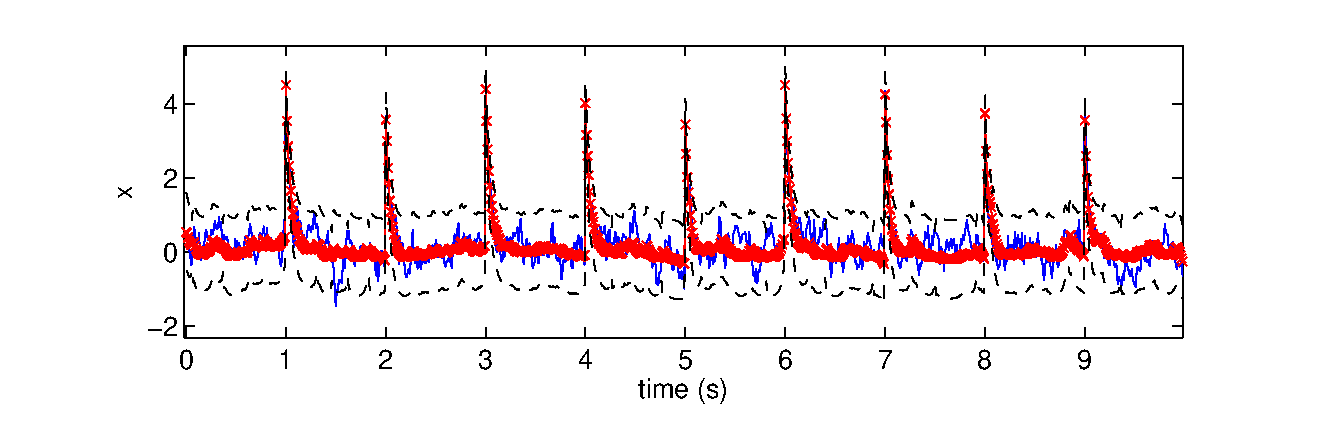
\includegraphics[width =
% 6in]{./stateVB.eps}
%
% \end{center} \caption{True state (solid blue line) and mean estimated state (marked red line). The
% true state lies consistently within the 99\% confidence intervals (dashed black line).}
% \label{fig:stateVB} \end{figure}
% 	

\begin{figure}[ht]
\begin{center}
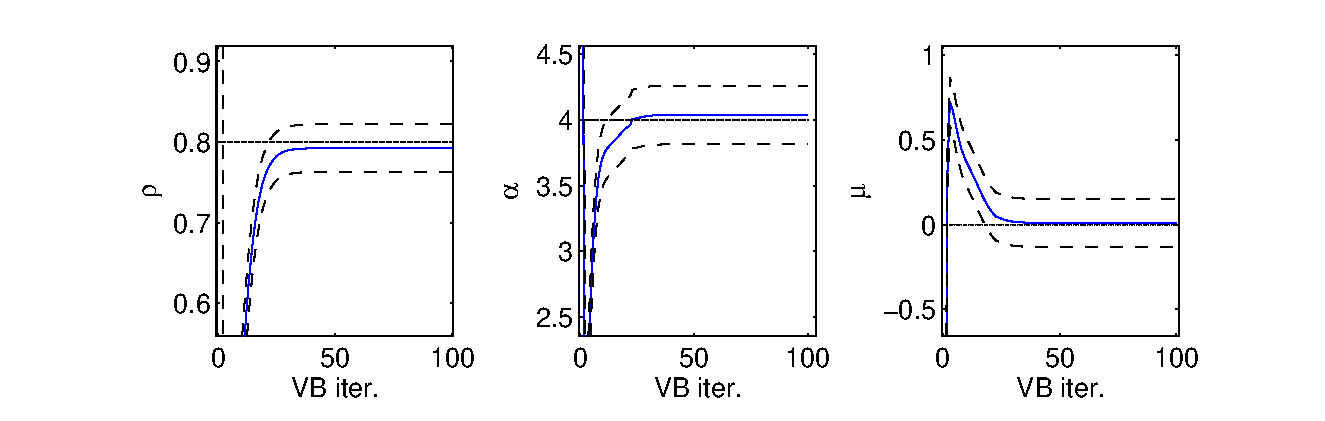
\includegraphics[width = 5.5in]{./Figures/parVB.eps}
\caption{Mean estimates and $99\%$ confidence intervals over 100 VB-EM iterations. The
parameters (including $\betab$ which is not shown) converge in distribution to reasonable estimates
independent of initial conditions.} \label{fig:parVB}
\end{center}
\end{figure}

We then compared our results to those obtained using EM \cite{Smith_2003} and those given by a Gibbs sampler on the same data set. To avoid identifiability issues, we also ran experiments with $\betab$ fixed to its true value. Table~\ref{tab:Parest} shows that all methods are
effective in estimating parameters for this data, with Gibbs and VB-EM also providing confidence
intervals which are in good agreement with the true values. It took 5s for the EM algorithm (50 iterations), 12s for the VB-EM algorithm (50 iterations), and 279s for the Gibbs sampler (5000 iterations) to converge.\footnote{Simulations
carried out on an Intel\textregistered Core\texttrademark 2 Quad Q6600 @ 2.40GHZ with 4GB of RAM}
	
\begin{table}[t] \caption{Parameter estimation by the EM algorithm, Gibbs sampler and VB-EM
	algorithm. Unless stated, $\betab$ was fixed to the true value during simulation.}
	\label{tab:Parest} \begin{center} \begin{tabular}{c|c|c|c|c|c} $\theta$
		&{\bf True}  	&{\bf EM} &{\bf Gibbs}  &{\bf VB-EM} &{\bf VB-EM} (free $\betab$) \\
		\hline &&&  \\[-2ex]
		$\rho$ 		&	0.80	&0.82	  & 0.79 $\pm$ 0.06 & 0.79 $\pm$ 0.03	  &	0.79 $\pm$ 0.03	 \\
		$\alpha$ 	&	4.00		&4.08	  & 3.81 $\pm$ 0.48	 & 4.04 $\pm$ 0.22	  &	4.07 $\pm$ 0.22   \\
		$\mu $		&	0.00	&-0.19	& 0.06 $\pm$ 0.24	 & 0.01 $\pm$ 0.14	&	0.02$\pm$ 0.14	 \\
		avr($\betab$)	&	1.00&  -	&         -		&	        -         &	0.99 $\pm$ 0.19	\\
\end{tabular} \end{center}
	\end{table}

A more informative test of the model's performance is its ability to capture the spike train
distribution. A quantitative measure of this can be achieved using the time-rescaling theorem of
\cite{Brown_2002} in conjunction with a Kolmogorov-Smirnov (KS) test, following the same procedure
as ~\cite{Smith_2003,Barbieri_2005}.  As a goodness of fit measure we found the mean squared maximum
distance between the model rate and the true rate over all output channels. The results for this KS
measure on a synthetic data set are given in Table~\ref{tab:MSE}; for completeness we also compare
with a sliding window (SW) empirical rate-estimator of 100ms width which is often used in these
applications \cite{Riehle_1997}. The Bayesian methods (VB-EM and Gibbs sampler) are seen to obtain a
considerable better goodness of fit than the EM algorithm (which in turn is much better than the
simple SW heuristic), indicating that retaining distributional information over the parameters does
lead to an improvement in the modelling of the spike distribution. To further validate the result we
ran a 2-sample t-test on the KS-measures from 20 different data sets. The mean-square maximum KS
distance for all these runs was 0.0070 for the VB-EM algorithm (fixed $\betab$) and 0.0089 for the
EM algorithm (also with fixed $\betab$). The test rejected the null hypothesis that the decrease in
error occurred by chance at the 5\% significance level.

\begin{table}[h] \caption{Mean squared maximum KS distances for the 20 neurons with different
	event-rate models (lower is better) for one data set. Unless stated, $\betab$ was fixed to
	the true value during simulation.} \label{tab:MSE} \begin{center}
		\begin{tabular}{c|c|c|c|c|c|c} &{\bf Gibbs} &{\bf VB-EM} &{\bf EM}  & {\bf VB-EM}
			(free $\betab$)  & {\bf EM} (free $\betab$) &{\bf SW} \\ \hline &&&
			\\[-2ex] {\bf MSE}  & 0.0046 & 0.0055 & 0.0076  & 0.0077  &  0.0136 & 0.0336
			\\ \end{tabular} \end{center} \end{table}




% \subsection{Online parameter tracking of a parameter from point process
% observations}\label{sec:OLres}
%
% Online state estimation and parameter monitoring can be useful in several applications, for
% instance in heart monitoring or in cases where electrical activity from spiking neurons are
% recorded in real-time. We applied the online VB filter of Section \ref{sec:OL} to the same example
% discussed previously. The nature of the data typical in these types of models required some
% further intervention for correct estimation using the online filter. In the absence of hidden
% state, the observed events in the output are due to the background firing rate $\mu$ and there is
% little or no information about $\rho, \alpha$ and $\betab$ in these regions. On the other hand,
% the hidden state governs the output in regions when it is substantial, that is, in time intervals
% close an input spike. In these areas there is significant information about $\rho, \alpha$ and
% $\betab$. We hence chose to update our parameter distributions only in regions where there is
% ample information about the relevant parameters. This was found to facilitate convergence and
% overall performance.
%
% For this study we assumed $C=80$ and that $\betab$ and $\mu$ were pre-determined from a previous
% offline analysis and assumed to be constants.  The choice of the forgetting factors was carried
% out by trial and error such that a parameter change could be tracked without compromising
% stability in the online estimates. We subsequently chose $\lambda^\rho = 0.8$ and $\lambda^\alpha
% = 0.8$. The result for the successful tracking a sudden change in the true value of $\rho$ from
% 0.8 to 0.6 is shown in Fig.~\ref{fig:oltrack}.
%
% \begin{figure}[h] \begin{center} 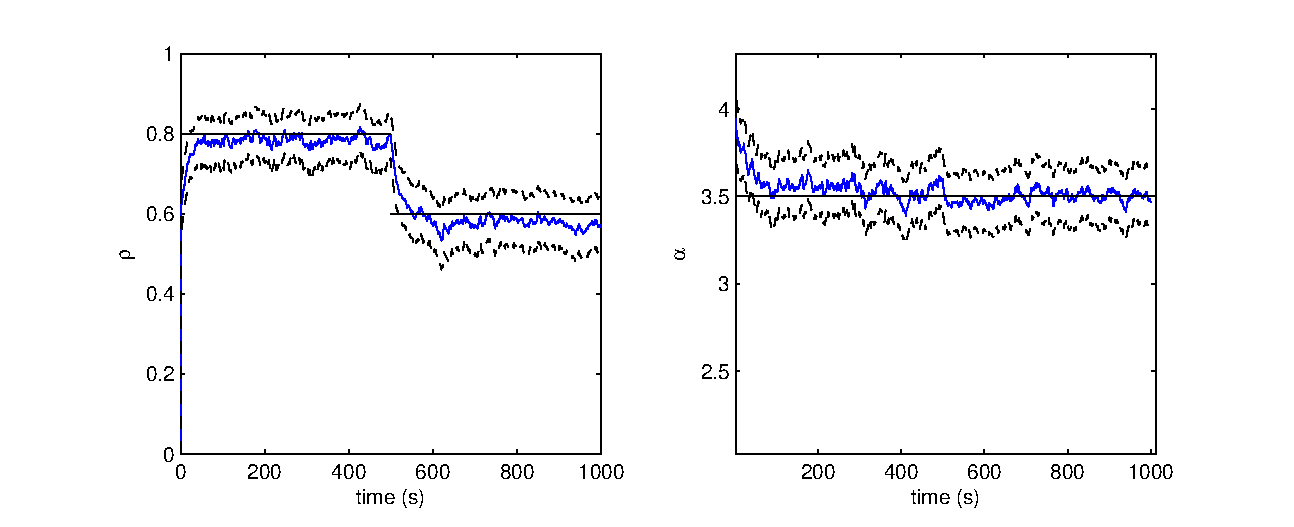
\includegraphics[width = 6in]{./onlinetrack.eps} \end{center}
% \caption{Online tracking of sudden change in parameter the true parameter (level black line)
% $\rho$ at time $t = 500s$. In this example $\mu$ and $\betab$ where assumed constant and known
% from previous offline analysis of the system. Note how the change in the estimate (tracking blue
% line) $\rho$ causes a slight change in the behaviour of the estimate of $\alpha$. This is expected
% from the assumed correlation between the two variables. The 99\% confidence intervals (black
% dashed lines) are seen to enclose the true value upon the filter reaching a steady behaviour.}
% \label{fig:oltrack} \end{figure}

% \subsection{Quantitative modeling of an L5 pyramidal cell}
%
% Here we demonstrate the use of offline VB-EM for the inference of a single ($C$ = 1) L5 pyramidal
% cell of a Wistrar rat, the data which was collected primarily for spike timing
% prediction~\cite{Gerstner_2009}. Despite the nature of the input being continuous (opposed to
% spikes) and the infrequency of the output spikes, we saw that the offline VB-EM algorithm was
% capable of converging to a model which manages to adequately represent the underlying data.
%
% The state covariance $\sigma^2_\epsilon$ was set to 0.0001 and we extracted the spikes from the
% data by detecting when a rising voltage crosses the zero threshold (as indicated in the
% competition guidelines). We estimated distributions over $\alpha, \rho, \mu, \betab$ and $\X_K$
% using the VB-EM algorithm. The predicted firing rate using the means of these distributions is
% shown in Fig.~\ref{fig:RDFR}. Despite it lying outside the confidence intervals in some instances,
% the Kolmogorov-Smirnov test in Fig.~\ref{fig:KSRD} indicates a relatively good agreement between
% the actual rate described by the data and the rate given by the model. The test corroborates the
% firing rates shown of Fig.~\ref{fig:RDFR}.
%
% \begin{figure}[h] \begin{center} %\framebox[4.0in]{$\;$} \subfigure[]{ 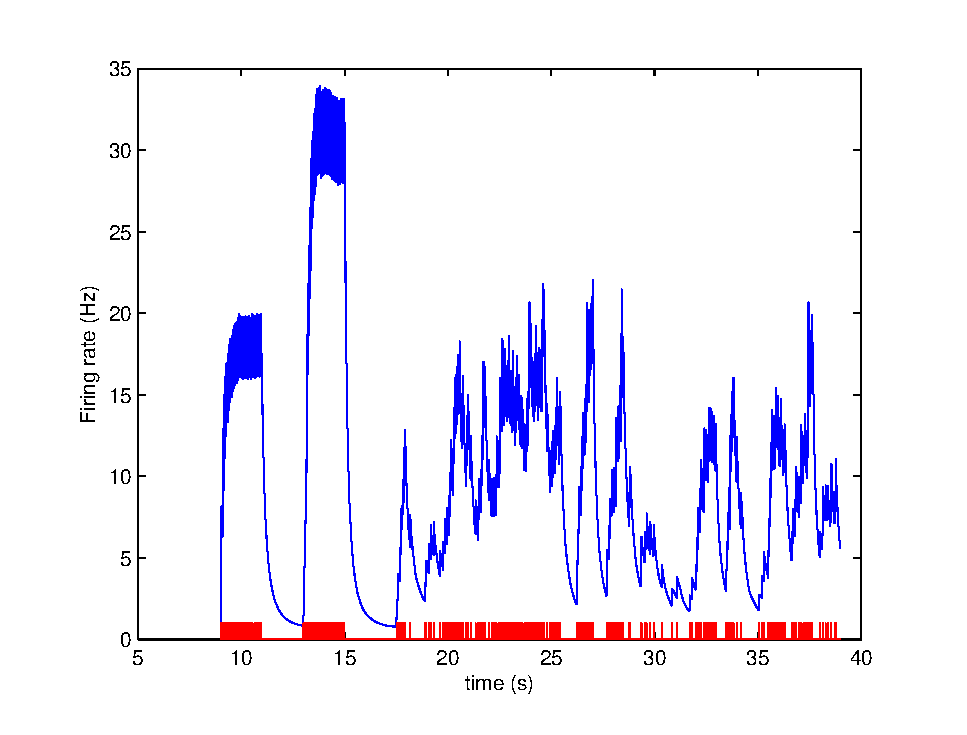
\includegraphics[width =
% 2.5in]{./Firingrate.eps}  \label{fig:RDFR}} \subfigure[]{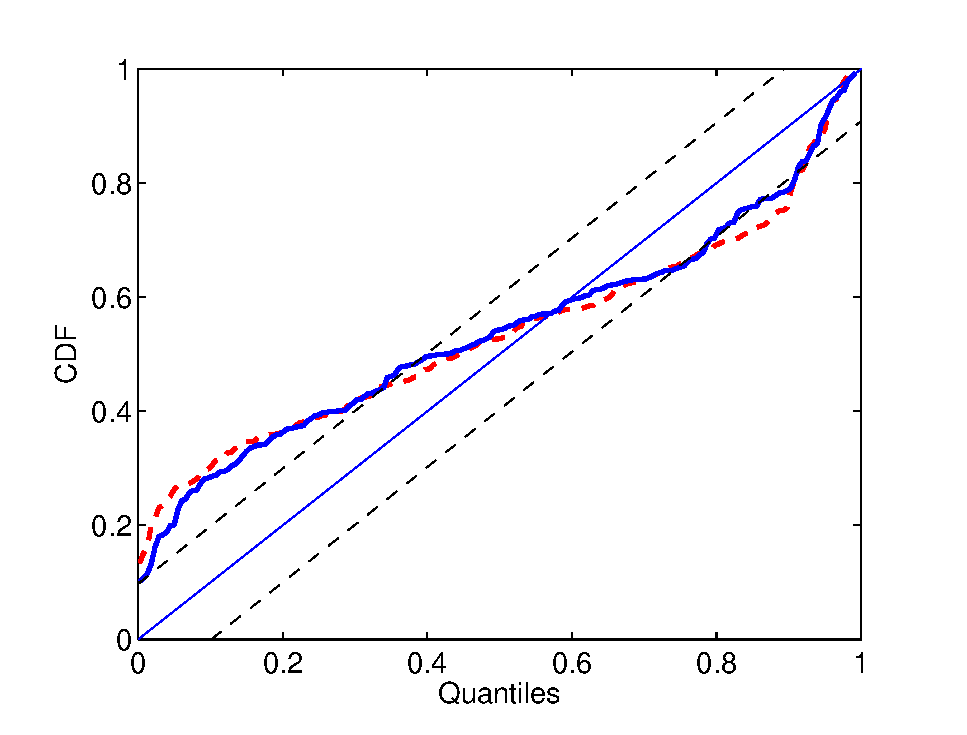
\includegraphics[width =
% 2.5in]{./KSRD.eps}  \label{fig:KSRD}} \caption{(a) Estimated firing rate $\lambda\Delta$ for the
% L5 pyramidal cell using VB-EM. The red spikes at the bottom indicate the spiking events. (b)
% Kolmogorov-Smirnov goodness-of-fit analyses for spiking rate inference of a single L5 pyramidal
% set, comparing the VB-EM rate estimate (solid blue line) to the EM rate estimate (dashed red line)
% and the 45 degree line indicating a perfect match between the model and the data.} \end{center}
%
% \end{figure}


\subsection{Online characterisation of taste stimuli}

As an example application of our online algorithm on real data, we model spiking patterns of
taste-response cells in the nucleus tractus solitarii (NTS) of Sprague-Dawley rats following the
application of different taste stimuli \cite{Lorenzo_2003}.  The attraction of the online approach
is that it provides a method for stimulus chemical discrimination by tracking changes in underlying
parameters upon the presentation of different stimuli.  The experimental data was obtained from
trials where different compounds dissolved in distilled water were delivered to the oropharyngeal area. Taste-evoked spike train data used in this study was delivered via neurodatabase.org - a neuroinformatics resource funded by
the Human Brain Project. From the data it was evident that a cell's response varies according to the stimulus applied in many ways. In some cases, monitoring the overall background activity through the parameter $\mu$ is sufficient to discriminate between two compounds. Sometimes the discrimination can be aided by also looking at the \emph{immediate} response of the cell to the stimulus. This entails the monitoring of the input gain $\alpha$, which modulates the state response to the input and hence controls the behaviour of the immediate response to the stimulus. We consider one cell from the data set and its response to three dissolved compounds; HCl, quinine and sucrose.


%For instance one cell's repsonse to sucrose was significantly less active overall than that to HCl, suggesting that by monitoring $\mu$ (background rate) one would be able to detect this change and hence identify the new presented compound. The overall response to quinine was slightly closer to that to HCl. However the \emph{immediate} response to quinine was much more substantial than that to HCl, suggesting a possibility


\begin{figure}[h] \begin{center}
%\framebox[4.0in]{$\;$}

\subfigure[Change in $\mu$ indicating a change in stimulus
 from HCl to sucrose and back to HCl. The parameter \newline change is indicative of a change in the spike train pattern (inset) when the stimulus is changed. ]{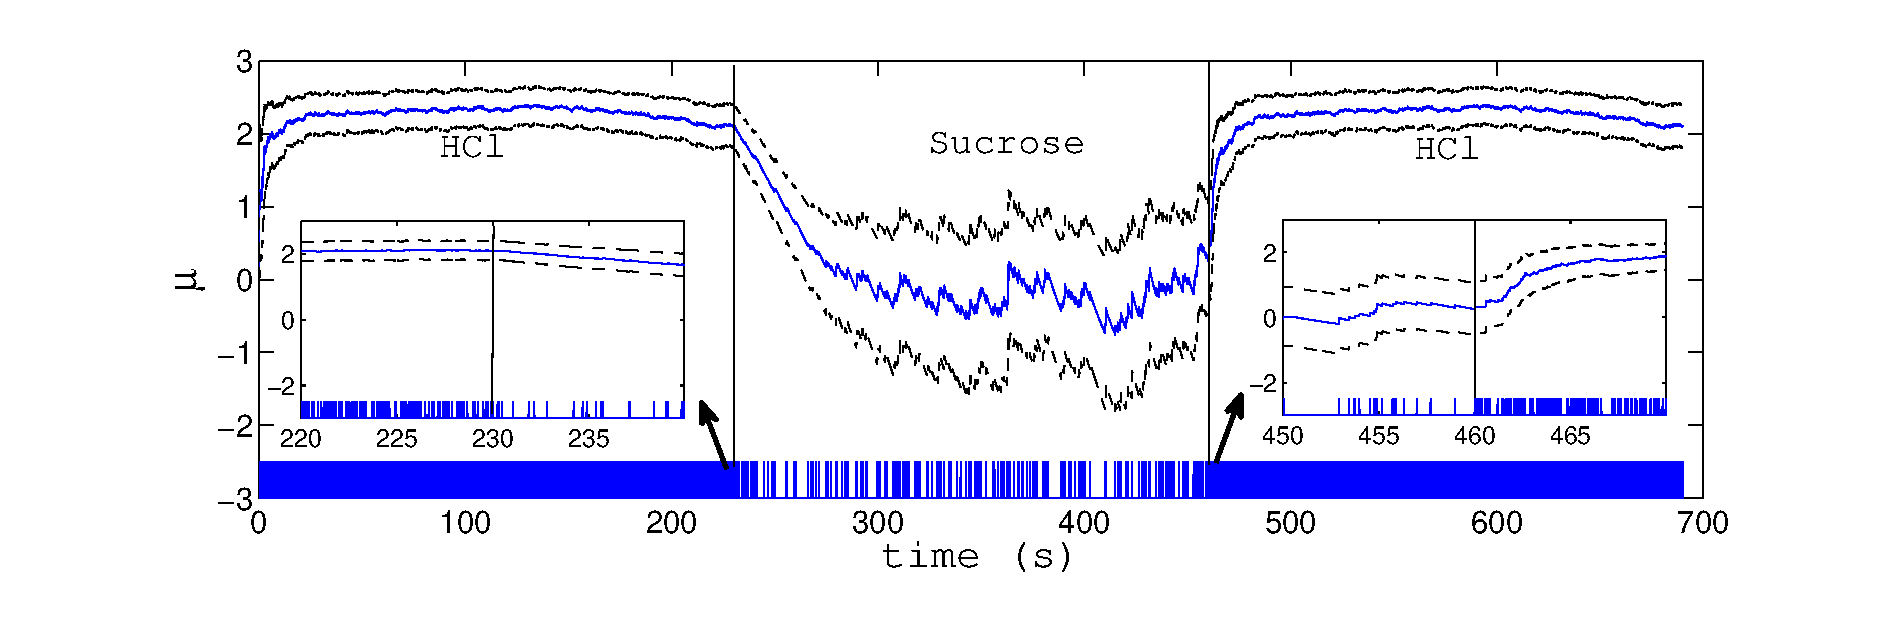
\includegraphics[width = 5.5in]{./Figures/HSH.eps}
 \label{fig:Sucrose}}
  \subfigure[Change in $\alpha$ and $\mu$ indicating a change of stimulus from HCl to quinine. Although the cell is, overall, less responsive to quinine ($\mu$), the immediate effect of its application is more substantial than in the case of HCl ($\alpha$).]{ 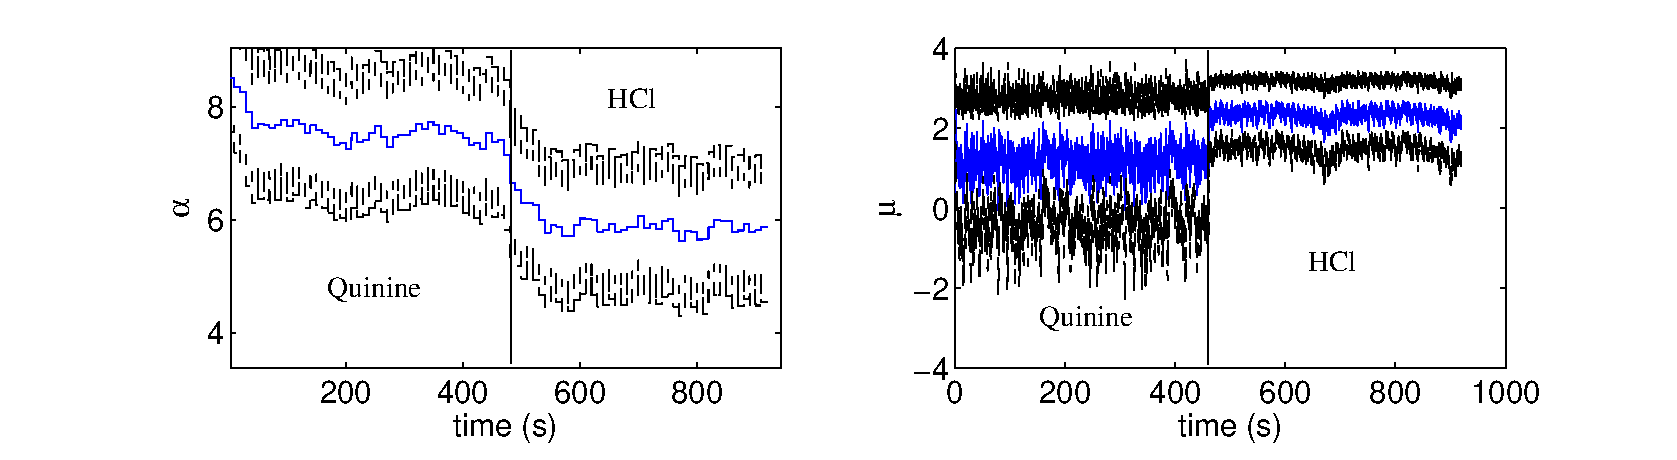
\includegraphics[width =
 5.5in]{./Figures/Quinine2HCl.eps}  \label{fig:Quinine}}
 \caption{Monitoring the change in spike response of one specific NTS cell. In both
 cases the solid vertical lines indicate where the change in applied chemical stimulus took place.}
 \label{fig:tastants} \end{center} \end{figure}

Although trials were separated by rinsing and a 1.5min wait we only considered the first 10s after the application of each stimulus and, for convenience, subsampled by a factor of 10, and concatenated these 10s batches of each trial together into one spike train. We then created an input spike train representative of the application of each tastant, and found indicative values for the unknown parameters using the offline VB-EM algorithm.  For all experiments we chose to fix $\rho = 0.96, \beta = 0.5$ and $\sigma^2_\epsilon = 0.1$.

From the spike train data, it was evident that the cell's response to sucrose was significantly less active overall than that to HCl, suggesting that by monitoring $\mu$ (background rate) one would be able to detect this change and hence identify the new presented compound. We fixed $\alpha = 5$ and then applied the online VB algorithm to a concatenated data set of spike trains generated in response to the two chemicals. As seen in Fig.~\ref{fig:Sucrose}, the change in $\mu$ on a change of stimulus was very evident. The cell's \emph{immediate} response to quinine was much more substantial than that to HCl and we hence jointly estimated $\alpha$ and $\mu$ from the corresponding concatenated data set. As seen from Fig.\ref{fig:Quinine}, both the change in $\alpha$ and that in $\mu$ was very evident. It is interesting to note that although the overall rate is lower for quinine than for HCl ($\mu$), the immediate stimulus response is larger ($\alpha$). The  behaviour of the immediate response to chemical stimuli is not apparent when using standard techniques which focus on overall firing rate~\cite{Lorenzo_2003}.

The dual online filter was robust and resistant to changes in state noise and fixed parameter
estimates. To ensure identifiability, the online parameter updates were carried out only in the
regions where ample information is present, so that $\alpha$ was only updated in regions close to
the application of the input (hence the step-like behaviour in Fig.~\ref{fig:Quinine}) and $\mu$ in regions between the
application of the respective inputs. This procedure is standard in online filtering in other areas,
e.g.  speech enhancement by spectral subtraction, in which noise levels are estimated in regions of the
signal where speech is not present~\cite{Boll_1979}. We show the filtered state and output probability of a spike occurring for a fourth compound, NaCl, in Fig.~\ref{fig:onlinestate}.

\begin{figure}[h] \begin{center}
%\framebox[4.0in]{$\;$}
 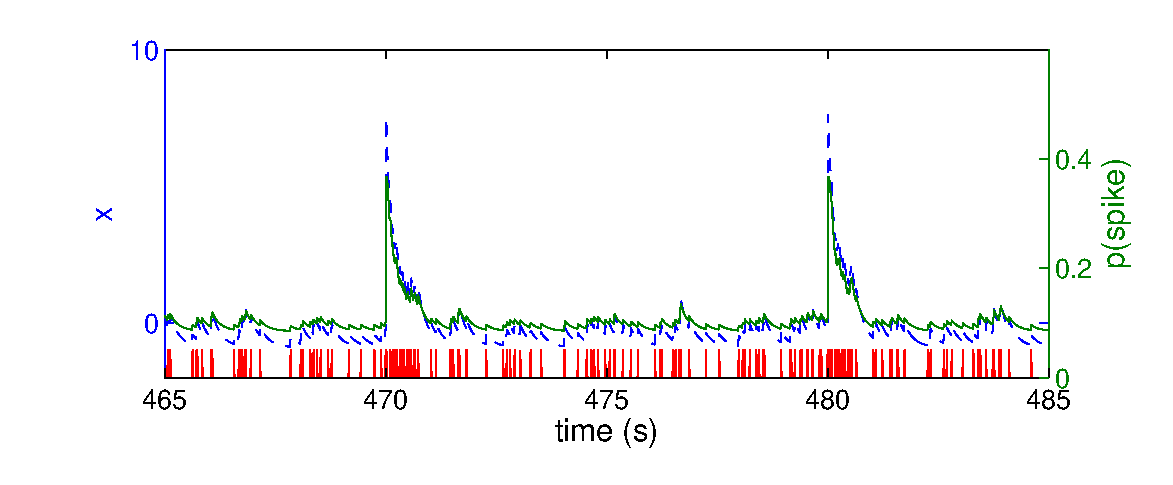
\includegraphics[width = 5in]{./Figures/taste_state.eps}  \caption{Estimated state (dashed blue) and
 probability of spike occurring (green) for when NaCl is being applied to the sensory cell every
 10s. Note how the probability is indicative of the frequency of spike events (red).}
 \label{fig:onlinestate} \end{center}

\end{figure}


\section{Discussion}

In this contribution, we proposed a variational Bayesian method for filtering and smoothing within
state-space models with point process observations. This class of models, introduced by Smith and
Brown \cite{Smith_2003}, provides a physiologically plausible signal processing framework for
event-based observations, and has proved a popular framework for analysing and decoding spike-train
data. Experiments on realistic simulated data show that the Bayesian treatment (either by VB or by
computationally expensive sampling methods) does indeed lead to an improvement in the modelling of
the spike train distribution, while retaining very good accuracy in estimating the parameter
posteriors. A major contribution of this work is the introduction of an online estimation framework.
This allows considerable computational savings, potentially paving the way for real-time biomedical
application. It also enables to monitor online changes in mode of operation of the system, as
exemplified in our case study of neural responses to different taste stimuli.

The application to online tracking suggests naturally an extension to consider state-space models
with switching parameters, which would formally incorporate into the model abrupt changes in mode of
operation. These have proved a popular tool in biomedical applications (see {\em e.g.}
\cite{Quinn_2008}), although the additional complexity is likely to come at some computational cost.
A further interesting extension would be to improve on the observation model by using more advanced
models for spike generation, such as integrate and fire; parameter estimation within these models
has recently been explored using search-type algorithms \cite{MacGregor_2009}, but the complexity of the likelihood model means
that it is likely that considerable work will be needed before they can be used in signal processing
applications.
%This work suggests several improvements over current methods used for dual state-parameter
%estimation in systems governed by state-space models with point process observations. First, the
%variational methods allow for the use of parameter second moments in estimating the hidden state,
%so that there is a decreased loss in information when compared to the parameter point estimate
%approximation of EM. The result is an improved model rate estimate as seen in the KS tests. Second,
%we present a dual \emph{online} state-parameter estimator which could be readily used for online
%parameter monitoring. This online algorithm is of considerable interest as it can also provide
%parameter uncertainty in real-time and we are currently looking into ways in which it can be
%adapted more for point-process information.

%Finally, in this work we have shown how the described point process model with the chosen
%conditional intensity function $\lambda$ can be used to for inferring states and parameters from
%real neural data. It is likely that there are better models to represent these observations,
%however the techniques presented here can in principle be applied to most state-space models of
%this form.




\bibliography{./spikeSSM}

\vfill

\end{document}
